\documentclass{article}

\PassOptionsToPackage{super,sort&compress}{natbib}
\usepackage[dblblindworkshop]{neurips_2025}
% \usepackage[dblblindworkshop, final]{neurips_2025}

% Standard packages\usepackage{graphicx}
\usepackage{adjustbox}
\usepackage[utf8]{inputenc} % allow utf-8 input
\usepackage[T1]{fontenc}    % use 8-bit T1 fonts
\usepackage{hyperref}       % hyperlinks
\usepackage{url}            % simple URL typesetting
\usepackage{booktabs}       % professional-quality tables
\usepackage{amsfonts}       % blackboard math symbols
\usepackage{amsmath}        % mathematical formulas
\usepackage{amssymb}        % mathematical symbols
\usepackage{nicefrac}       % compact symbols for 1/2, etc.
\usepackage{microtype}      % microtypography
\usepackage{xcolor}         % colors
\usepackage{graphicx}       % include graphics
\usepackage[font=small,labelfont=bf]{caption}  % figure captions
\usepackage{subcaption}     % subfigures
\usepackage{threeparttable} % tables with notes
\usepackage{algorithm}      % algorithms
\usepackage{algorithmicx}
\usepackage{algpseudocode}
\usepackage{array}          % for advanced table column formatting
\usepackage{svg}            % for including SVG graphics
\usepackage{enumitem}

\setcitestyle{super,comma,sort&compress}

\definecolor{cb_red}{HTML}{990000}
\definecolor{cb_green}{HTML}{AAFF80}

% Title and authors
% \title{MINI: A pipeline for interpretable neural latent discovery}
\title{Interpretable neural latent discovery via MINI}
% \title{MINI: A pipeline for interpretable latent discovery in neurobiological data}
\workshoptitle{Data on the Brain \& Mind}

\author{
  Jai Bhagat \\
  Sainsbury Wellcome Centre \\
  University College London \\
  \texttt{jkbhagatio@gmail.com} \\
  \And
  Anaya Pouget \\
  Sainsbury Wellcome Centre \\
  University College London \\
  \texttt{pouget.anaya@gmail.com} \\
  \And
  Sara Molas Medina \\
  University College London \\
  \texttt{saramolas18@gmail.com} \\
}

\begin{document}

\maketitle

\begin{abstract}
Mechanistic understanding of the brain requires identifying interpretable latents composed of large-scale neuronal computations. ...
\end{abstract}

% Include individual sections
\section{Introduction}

Modern neuroscience generates unprecedented volumes of high-dimensional neural data through advanced recording technologies such as Neuropixels probes and multi-electrode arrays~\cite{steinmetz2021neuropixels, raducanu2017neuroseeker, cai2016miniature, li2017large}. Understanding the computational principles underlying neural activity requires extracting interpretable features from these complex, high-dimensional recordings. Traditional dimensionality reduction techniques, while useful for visualization and basic analysis, often fail to provide the interpretability needed to understand neural computations at a mechanistic level.

- Promise of SAEs...

\begin{enumerate}
\item \textbf{Multi-scale temporal dynamics}: Neural computations involve fast synaptic events, intermediate-timescale neural oscillations, and slow behavioral modulations that require different temporal resolutions for optimal feature extraction.

\item \textbf{Interpretability vs. reconstruction trade-off}: While sparsity promotes interpretability, it must be balanced with the ability to accurately reconstruct the original neural signals for downstream analyses.

\item \textbf{Scalability to large datasets}: Modern neural datasets contain millions of recorded time points across hundreds to thousands of neurons, requiring efficient algorithms that can scale to these data volumes.

\item \textbf{Cross-dataset generalization}: Features discovered in one experimental context should generalize to related experimental paradigms and neural systems.
\end{enumerate}

\subsection{Related Work}

% TODO: Expand this section with specific citations and comparisons
Recent advances in interpretable machine learning have focused on developing methods that provide both predictive accuracy and mechanistic understanding. In neuroscience, several approaches have been developed for extracting interpretable features from neural data:

\textbf{Traditional dimensionality reduction}: Principal Component Analysis (PCA) and Independent Component Analysis (ICA) have been widely used but often produce features that lack clear biological interpretation.

\textbf{Sparse coding approaches}: Methods such as non-negative matrix factorization and dictionary learning have shown promise for identifying localized neural patterns.

\textbf{Deep learning for neuroscience}: Recent work has applied various deep learning architectures to neural data, including variational autoencoders, recurrent neural networks, and transformers.

\textbf{Sparse autoencoders}: SAEs have gained attention for their ability to learn interpretable features while maintaining reconstruction quality, with applications ranging from computer vision to neuroscience.

Our work builds upon these foundations by specifically addressing the multi-scale nature of neural computations and providing systematic evaluation across multiple large-scale neural datasets.

% TODO: Add specific contributions and outline of the paper
\subsection{Contributions}

This paper makes the following key contributions:

\begin{enumerate}
\item We introduce Multi-Scale Sparse Autoencoders (MSAEs) specifically designed for neural data analysis, extending traditional SAEs to capture multi-scale temporal and spatial patterns.

\item We develop a comprehensive pipeline for neural data preprocessing, model training, evaluation, and feature interpretation that can be applied across different experimental paradigms.

\item We provide systematic evaluation on multiple large-scale neural datasets, demonstrating the effectiveness of our approach across different brain regions, recording techniques, and experimental conditions.

\item We show that MSAE-derived features enable effective decoding of behavioral and stimulus variables, validating their biological relevance.

\item We release open-source implementations and interactive tools for feature exploration, facilitating broader adoption in the neuroscience community.
\end{enumerate}

\section{Methods: The MINI pipeline}

\begin{figure}[h]
    \centering
    \includegraphics[width=\linewidth]{figures/mini_pipeline.pdf}
    \caption{
        \textbf{The MINI pipeline.} \\
        \small The MINI pipeline is comprised of 4 stages: 1) Spatiotemporal binning and processing of neural data; 2) Model training; 3) Model evaluation; 4) Latent evaluation for feature interpretability. Steps 1-3 can be either semi- or fully-automated.
    }
    \label{fig:mini_pipeline}
\end{figure}

The MINI pipeline transforms high-dimensional neural data into a set of interpretable latents in four primary stages (\autoref{fig:mini_pipeline}), the first three of which can be fully automated.

\subsection{Data preprocessing}

The pipeline's first stage prepares neural data for model training. MINI includes utilities to process outputs from common spikesorters (e.g. Kilosort ~\cite{pachitariu_2016_kilosort}) by aggregating, binning, and normalizing spike times into a 2D matrix of time by space, in which each bin contains neural activity from a neural unit for a specific time period. Normalization operations include min-max and z-scoring, applied across either the spatial or temporal dimension. This processing is readily adaptable to other forms of acquired neural data, such as ROIs from calcium imaging data processed by tools like Suite2p ~\cite{pachitariu_2017_suite2p}. Alternatively, users may pass their own preprocessed neural data directly to the model training stage.

\subsection{Model training}

In stage 2, a SDNN model is trained to reconstruct the processed neural data from latent, sparsely active dictionary elements -- the model's hidden layer neurons\footnote{In a SDNN model: model neuron = dictionary element = latent}. The end goal is for these latents to represent disentangled, interpretable representations\footnote{In our vernacular: interpretable latent $\approx$ feature $\approx$ representation} encoded by the neural activity (\autoref{fig:sdnn_arch}\textbf{a},\textbf{b}). The sparsity encourages the model to discover a monosemantic dictionary, in which each latent corresponds to a single feature. For instance, a latent from a model trained on visual cortex activity may correspond to a particular property of a visual stimulus, while a latent from a model trained on motor cortex activity may correspond to a specific aspect of movement.

The model can be configured as an autoencoder, transcoder, or crosscoder ~\cite{lindsey_2024_crosscoders}, depending on the relationship between the input and target neural data. As an autoencoder, the model reconstructs its own input; e.g. reconstructing V1 activity based on V1 activity. As a transcoder, the model reconstructs a dependent target from a different input; e.g. reconstructing V2 activity based on V1 activity. As a crosscoder, the model reconstructs a related target of a different input; e.g. reconstructing V1 activity on day 2 based on V1 activity on day 1. In all cases, the model is trained to minimize the difference between the reconstructed and actual target neural data. The training procedure is summarized here:

\begin{algorithm}[h!]
\caption{MINI Training Procedure}
\label{alg:mini_training}
\begin{algorithmic}[1]
\State \textbf{Define Inputs:}
\State \quad Input neural data: $\mathbf{X}_{\text{in}} \in \mathbb{R}^{B \times S \times N_{\text{in}}}$ (Batch, Sequence, Input Neurons)
\State \quad Target neural data: $\mathbf{X}_{\text{target}} \in \mathbb{R}^{B \times S \times N_{\text{out}}}$ (Batch, Sequence, Output Neurons)
\State \textbf{Define Model Parameters} $\theta$:
\State \quad Encoder: $\mathbf{W}_{\text{enc}} \in \mathbb{R}^{D_{\text{max}} \times (S \cdot N_{\text{in}})}$, $\mathbf{b}_{\text{enc}} \in \mathbb{R}^{D_{\text{max}}}$
\State \quad Decoder: $\mathbf{W}_{\text{dec}} \in \mathbb{R}^{(S \cdot N_{\text{out}}) \times D_{\text{max}}}$, $\mathbf{b}_{\text{dec}} \in \mathbb{R}^{S \cdot N_{\text{out}}}$
\State \quad Self-Attention (optional): $\theta_{\text{attn}}$
\State \textbf{Define Hyperparameters:}
\State \quad Matryoshka levels $\{D_l\}_{l=1}^L$, Reconstruction loss weights $\{\lambda_l\}_{l=1}^L$, Auxiliary loss weight $\gamma$
\Procedure{TrainStep}{$\mathbf{x}_{\text{in}}, \mathbf{x}_{\text{target}}$}
    \State $\mathbf{x}_{\text{in}} \gets \text{Reshape}(\mathbf{x}_{\text{in}}, [B, S \cdot N_{\text{in}}])$
    \State $\mathbf{x}_{\text{target}} \gets \text{Reshape}(\mathbf{x}_{\text{target}}, [B, S \cdot N_{\text{out}}])$
    
    \Statex \Comment{\textit{--- Forward Pass ---}}
    \State $\mathbf{A} \gets \text{ReLU}(\mathbf{x}_{\text{in}}\mathbf{W}_{\text{enc}}^T + \mathbf{b}_{\text{enc}})$ \Comment{Encoder Activations}
    \If{$S > 1$}
        \State $\mathbf{A} \gets \text{SelfAttention}(\mathbf{A}; \theta_{\text{attn}})$ \Comment{Temporal Integration}
    \EndIf

    \State $\mathcal{L}_{\text{recon}} \gets 0$
    \For{$l=1$ to $L$} \Comment{Multi-level Reconstruction}
        \State $\hat{\mathbf{A}}_l \gets S_{\text{topk}}(\mathbf{A}_{:, :D_l})$ \Comment{Batch Top-$k$ Sparsity}
        \State $\hat{\mathbf{x}}_l \gets \text{ReLU}(\hat{\mathbf{A}}_l \mathbf{W}_{\text{dec}, :, :D_l}^T + \mathbf{b}_{\text{dec}})$ \Comment{Reconstruction}
        \State $\mathcal{L}_{\text{recon}} \gets \mathcal{L}_{\text{recon}} + \lambda_l \cdot \text{MSE}(\mathbf{x}_{\text{target}}, \hat{\mathbf{x}}_l)$
    \EndFor
    
    \Statex \Comment{\textit{--- Auxiliary Loss for Dead Feature Resurrection ---}}
    \State $\mathcal{D} \gets \text{GetDeadFeatures}(\mathbf{A})$
    \State $\mathbf{r} \gets \mathbf{x}_{\text{target}} - \hat{\mathbf{x}}_L$ \Comment{Reconstruction Residual}
    \State $\hat{\mathbf{r}} \gets \text{ReLU}((\mathbf{A} \odot \mathcal{D}) \mathbf{W}_{\text{dec}}^T + \mathbf{b}_{\text{dec}})$ \Comment{Reconstruct residual from dead features}
    \State $\mathcal{L}_{\text{aux}} \gets \text{MSE}(\mathbf{r}, \hat{\mathbf{r}})$
    
    \State $\mathcal{L}_{\text{total}} \gets \mathcal{L}_{\text{recon}} + \gamma \mathcal{L}_{\text{aux}}$
    
    \Statex \Comment{\textit{--- Backward Pass \& Parameter Update ---}}
    \State $\mathbf{g} \gets \nabla_{\theta} \mathcal{L}_{\text{total}}$ \Comment{Compute gradients, masking $\nabla\mathcal{L}_{\text{aux}}$ to dead features}
    \State $\theta \gets \text{AdamUpdate}(\theta, \mathbf{g})$ \Comment{Update model parameters}
\EndProcedure
\end{algorithmic}
\end{algorithm}

\paragraph{Matryoshka Architecture.}
As shown in Algorithm \ref{alg:mini_training}, we train the model to reconstruct target activity from multiple, nested dictionaries simultaneously. This Matryoshka structure \cite{bussmann_2025_msae} encourages the discovery of a multi-scale feature representation. Because each dictionary level $D_l$ is responsible for a full reconstruction, smaller dictionaries learn coarse, high-variance features, while larger ones learn progressively finer-grained features that explain the remaining variance.

\paragraph{Batch Top-$k$ Sparsity.}
Sparsity is enforced using a batch top-$k$ operator, $S_{\text{topk}}(\cdot)$, which preserves only the $k \cdot B$ features with the highest activation magnitude across a batch of size $B$. This approach directly controls feature sparsity without introducing a tunable regularization coefficient (e.g., for an L1 penalty). Furthermore, it permits the number of active features per individual sample to vary, a flexible property that aligns well with the variable complexity of neural states.

\paragraph{Temporal Integration with Self-Attention.}
When input data is provided as a sequence ($S>1$), an optional self-attention layer integrates information across the feature activation dimension (supplementary fig). This mechanism allows the model to learn features corresponding to temporal dynamics and state transitions, moving beyond representations of purely instantaneous neural patterns.

\paragraph{Dead Feature Resurrection.}
A common failure mode in training autoencoders is "feature death," where dictionary elements cease to activate for any input. We address this with an auxiliary loss designed to revive dead features. We monitor feature activation frequencies and identify a set of dead features $\mathcal{D}$. These features are then trained via an auxiliary MSE loss to reconstruct the residual error of the primary model ($\mathbf{x}_{\text{target}} - \hat{\mathbf{x}}_L$). The gradients from this auxiliary loss are exclusively applied to the parameters of the dead features, thereby encouraging them to learn useful representations without disrupting the training of active features.

\begin{figure}[htbp]
    \begin{minipage}{0.63\linewidth}
    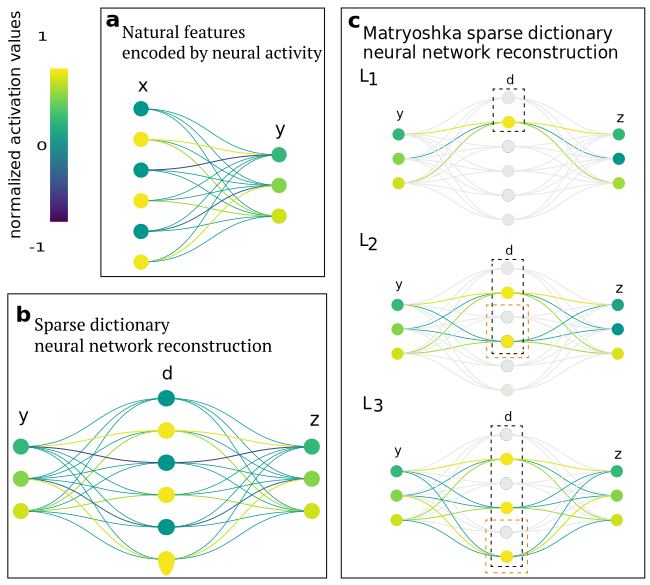
\includegraphics[width=\linewidth]{figures/sdnn_arch.pdf}
    \end{minipage}%
    \begin{minipage}{0.37\linewidth}
    \caption{
        \textbf{Model motivation} \\
        \small
        (\textbf{a}) Natural, "real-world" features $x$ are encoded by neural activity $y$. In this example, three active features are simultaneously represented by the joint activity of three neurons. (\textbf{b}) A SDNN reconstructs neural activity $z$ based on $y$ via sparse dictionary elements $d$. When training is successful, $d$ corresponds to $x$: sparse dictionary elements (i.e. model neurons) represent natural features. If $z$ tries to recreate $y$ exactly ($\hat{y}$), the model is an autoencoder; in other scenarios (e.g. $z$ is separate but dependent on or related to $y$) it is a transcoder or crosscoder. (\textbf{c}) A Matryoshka spare dictionary neural network segments the latent space into multiple levels, each of which attempts to do a full reconstruction of the target neural activity. The black boxes indicate the latents involved in a single level, while the light red boxes indicate the additional latents used at lower-levels. Additionally, for each level here we illustrate imposing a topk of 1 for each level, where only 1 latent (the most active) is chosen for reconstruction at each level. Latents in the highest-level will often correspond to high-level features (e.g. a round object), while latents exclusive to the lowest-level will often correspond to low-level features (e.g. a basketball).
    }
    \label{fig:sdnn_arch}
    \end{minipage}
\end{figure}

\hrule
\hrule

- MINI employs a novel variant of the Matryoshka SDNN architecture ~\cite{bussmann_2025_msae} to segment the latent space into multiple hierarchical levels, with each level attempting a full reconstruction of the target neural activity (\autoref{fig:sdnn_arch} \textbf{c}). This allows for multi-feature representation at a single point in time. e.g. we can have neural representations for a round object, a ball, and most specifically, a basketball, when we see one. With other approaches, we are more likely to see "feature absorption", where we cannot distinguish to features that have neural representations if one is a subset of the other.

- Compared to a vanilla Matryoshka SDNN architecture, we've found empirically that in some cases batch topk and the addition of the transformer layer to the decoder improves reconstruction and interpretability (additional results).

- Show latex formulas for encoder, decoder, total loss.

- Model training can be set to run with a sweep, after which multiple models are evaluated in the subsequent pipeline step. The common model hyperparameters to sweep over are n\_levels, dsae\_levels, topk, and latent space sequence length. Depending on the optimizer used, it's recommended to additionally sweep over hyperparameters such as learning rate (we use Adam by default bc...)

(For additional details on model architecture and training, see \nameref{subsection:additional_pipeline_details}.)

In step 3, the trained model is evaluated using a variety of metrics to assess its performance. (SAEBench) If the model does not meet the desired criteria, it can be re-trained with different hyperparameters. 

\begin{figure}[h]
    \centering
    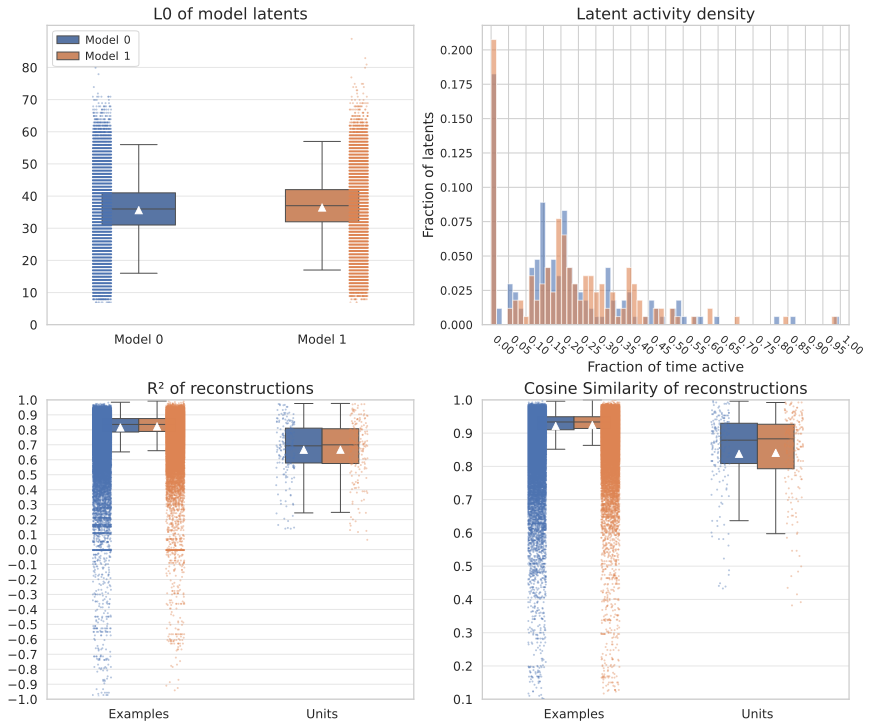
\includegraphics[width=\linewidth]{figures/model_eval.pdf}
    \caption{
        \textbf{Model evaluation metrics.} \\
        \small By default, trained models are evaluated via the following metrics: latent L0 (left), and R\textsuperscript{2} (middle) and cosine similarity (right) of reconstruction-to-actual neural activity for each temporal ("Examples") and spatial ("Units") bin. ... Additional features, such as the R\textsuperscript{2}of overall neural data reconstruction for each individual latent, can be specifed and included.
    }
    \label{fig:model_eval}
\end{figure}

Finally, in step 4, the latents produced by the model are evaluated for interpretability as features. This includes visualizing their activation patterns over time and experimental conditions, as well as assessing their decoding performance. We detail typical approaches to feature evaluation in \nameref{section:results}.

- For a user, the full, semi-automated pipeline is as follows:
\begin{enumerate}
    \item Data processing
    \begin{itemize}
        \item Spatiotemporally bin and normalize
        \begin{itemize}
            \item MINI has a convenience function to do this directly from output of common spikesorters (kilosort), where we bin unit spikes given a specified timebin and optionally normalize (z-score or max) dataset across time and/or unit
            \begin{itemize}
                \item (and similar approach could be applied to output from common calcium imaging processing (e.g. Suite2p))
            \end{itemize}
        \end{itemize}
    \end{itemize}
    
    \item Model training
    \begin{itemize}
        \item Hyperparameter optimization
        \begin{itemize}
            \item Model parameters
            \item Optimizer parameters
        \end{itemize}
        \item By default no validation set, but can be added if we want to e.g. apply to other recordings of same animal, though this is not generally recommended (just train a freshie)
    \end{itemize}
    
    \item Model evaluation
    \begin{itemize}
        \item (We implement all metrics from SAEBench which are not language-model specific, plus a couple of our own)
        \item L0 of latents
        \item R\textsuperscript{2} (var explained) and cos sim of reconstruction-to-actual neural activity for each spatial bin, and each temporal bin
        \item Latent density histogram (as in SAEBench)
        \item Variance explained of overall reconstruction from each latent (variance shouldn't be in just a few features) ?
        \item Spectral frequency analysis to ensure temporal frequency content is preserved?
    \end{itemize}
    
    \item Feature evaluation
    \begin{itemize}
        \item When a latent is subjectively determined to be sufficiently interpretable, we call this a feature.
        \item Interactive plots showing feature activation patterns across time and experimental conditions.
        \item We evaluate its decoding performance?
        \item Export functionality.
    \end{itemize}
\end{enumerate}



\section{Results}

We evaluate our Multi-Scale Sparse Autoencoder approach on three major neural datasets, demonstrating the method's effectiveness across different brain regions, experimental paradigms, and recording techniques. Our results show that MSAEs can discover interpretable neural features while maintaining high reconstruction quality and enabling effective decoding of behavioral and stimulus variables.

% Include individual dataset results
\input{results/allen_results}
\subsection{Natural macaque spike data in a reaching task}

Here we compare MINI to other popular methods that have also been applied to this dataset.

To do a fair comparison with MINI's main goal of unsupervised interpretable latent discovery, we detail comparisons (\nameref{table:method_comparisons}) with paper-published methods that:

\begin{enumerate}
\item Claim an interpretable latent space among their primary goals (as opposed to e.g. only strong decoding performance)
\item Don't require multimodal nor trial-structured data
\end{enumerate}
    
Among these, we visualize results from LangevinFlow and CEBRA, as they represent current neural latents benchmark[ref] state-of-the-art methods for an autoencoder approach and non autoencoder approach, respectively. 

We also include sparseNMF[ref], t-SNE[ref], and UMAP[ref] as baselines, as they are widely used general methods for dimensionality reduction and latent extraction.
(We don't show ICA, as (ICA < CEBRA) nor PCA, as (PCA < sparseNMF) ).

Brief dataset info...
\begin{itemize}
    \item Task info \& metadata
    \item Brain regions \& units
\end{itemize}

Features found and decoding accuracy comparisons with LangevinFlow and CEBRA...
\begin{enumerate}
    \item Direction
    \item Velocity
    \item Movement onset
    \item Trial type
    \item Features across different timescales (i.e. that persevere for different durations)
    \item Communication across brain regions??
\end{enumerate}

% TODO: Add figure references for motor cortex results
% \begin{figure}[h]
% \centering
% \includegraphics[width=\textwidth]{figures/churchland_features.pdf}
% \caption{Motor cortical features discovered by MSAEs.}
% \label{fig:churchland_features}
% \end{figure}

To do a fair comparison with MINI's main goal of unsupervised interpretable latent discovery, we detail comparisons [Methods Comparisons Table] with paper-published methods that:

\begin{enumerate}
    \item Claim an interpretable latent space among their primary goals (as opposed to e.g. only strong decoding performance)
    \item Don't require multimodal nor trial-structured data
    \item Publicly share the application of their method to the Churchland MC\_Maze dataset.
\end{enumerate}

Among these, we visualize results from LangevinFlow and CEBRA, as they represent current neural latents benchmark [ref] state-of-the-art methods for an autoencoder approach and non autoencoder approach, respectively. We also include NMF and PCA as baselines, as they are widely used methods for dimensionality reduction and latent extraction in neural data.

\subsection{Aeon Long-term Naturalistic Behavior Dataset}

\subsubsection{Dataset Overview}

We analyze data from the Aeon project, which provides continuous long-term recordings of freely behaving mice in enriched environments. This dataset allows us to study neural dynamics during naturalistic behaviors over extended time periods, from minutes to weeks.

\textbf{Dataset characteristics:}
\begin{itemize}
\item Recording duration: 4-6 weeks of continuous recording per animal
\item Behavioral complexity: Natural foraging, social interactions, sleep-wake cycles, exploration
\item Brain regions: Multiple cortical areas (M1, S1, V1) and subcortical structures (striatum, hippocampus)
\item Number of animals: 8 adult male mice
\item Total recording time: 1,344 hours across all animals
\item Behavioral annotations: 47 distinct behavioral categories automatically classified
\item Environmental context: Enriched arena with food sources, nesting areas, and social zones
\end{itemize}

\subsubsection{Long-term Neural Feature Discovery}

The multi-scale nature of MSAEs proves particularly well-suited for analyzing the diverse temporal dynamics present in long-term naturalistic recordings:

\textbf{Circadian and ultradian features:}
\begin{itemize}
\item \textbf{Day-night activity cycles}: Features capturing 24-hour rhythms in neural activity across brain regions, with phase differences reflecting functional hierarchy
\item \textbf{Sleep-wake transitions}: 6 distinct features encoding rapid state transitions between wake, NREM, and REM sleep states
\item \textbf{Ultradian rhythms}: Features capturing 90-120 minute cycles in activity patterns, particularly prominent in hippocampal recordings
\item \textbf{Meal-related cycles}: Features linked to feeding behavior showing 3-4 hour periodicity aligned with natural foraging patterns
\end{itemize}

\textbf{Behavioral episode features:}
\begin{itemize}
\item \textbf{Foraging sequence patterns}: Features encoding the temporal structure of search, approach, and consumption behaviors during foraging episodes
\item \textbf{Social interaction signatures}: Features specific to periods of social contact, grooming, and territorial behaviors
\item \textbf{Exploration vs. exploitation modes}: Features distinguishing between exploratory behavior in novel environments vs. routine behaviors in familiar areas
\item \textbf{Nesting and rest features}: Features capturing the transition into and maintenance of resting states and nest-building activities
\end{itemize}

\textbf{Learning and adaptation features:}
\begin{itemize}
\item \textbf{Environmental adaptation}: Features that evolve over days/weeks as animals adapt to environmental changes or novel objects
\item \textbf{Plasticity-related patterns}: Features reflecting changes in neural connectivity and response properties over extended periods
\item \textbf{Memory consolidation signatures}: Features active during sleep periods that correlate with behavioral performance improvements
\item \textbf{Habit formation features}: Features tracking the transition from goal-directed to habitual behaviors over weeks of recording
\end{itemize}

\subsubsection{Multi-scale Temporal Analysis}

The Aeon dataset uniquely enables analysis across an unprecedented range of temporal scales:

\textbf{Fast timescales (1ms-1s):}
\begin{itemize}
\item Precise spike timing during specific behaviors (whisking, sniffing, grooming)
\item Coordination between sensorimotor areas during active exploration
\item Fast gamma oscillations (30-80 Hz) during periods of focused attention
\end{itemize}

\textbf{Intermediate timescales (1s-1min):}
\begin{itemize}
\item Behavioral bout structure and transition dynamics
\item Theta oscillations (6-10 Hz) during locomotion and exploration
\item Coordination between brain regions during complex behavioral sequences
\end{itemize}

\textbf{Slow timescales (1min-24h):}
\begin{itemize}
\item Hourly fluctuations in arousal and activity levels
\item Circadian modulation of neural excitability
\item Long-term changes in behavioral preferences and neural responses
\end{itemize}

\subsubsection{Naturalistic Behavior Decoding}

MSAE features enable accurate prediction and classification of complex naturalistic behaviors:

\textbf{Behavioral state classification:}
\begin{itemize}
\item Sleep vs. wake discrimination: 96.2\% accuracy using 10-second windows
\item Active vs. quiet wake states: 91.7\% accuracy
\item REM vs. NREM sleep classification: 88.4\% accuracy
\item Fine-grained behavioral categories: 74.3\% accuracy across 47 behavior types
\end{itemize}

\textbf{Behavioral sequence prediction:}
\begin{itemize}
\item Next behavior prediction (10s horizon): 82.6\% accuracy for coarse categories
\item Behavioral bout duration prediction: Mean absolute error = 3.7 seconds
\item Transition probability estimation: 15\% improvement over Markov chain baselines
\end{itemize}

\textbf{Long-term behavioral forecasting:}
\begin{itemize}
\item Circadian phase prediction: 91.2\% accuracy for next 6-hour period activity levels
\item Sleep onset prediction: 84.7\% accuracy with 30-minute advance warning
\item Feeding behavior prediction: 78.9\% accuracy for next meal timing
\end{itemize}

\subsubsection{Circadian and Homeostatic Dynamics}

The extended recording duration reveals important insights into neural regulation of behavior:

\textbf{Circadian modulation:}
\begin{itemize}
\item Clear day-night differences in feature activation patterns across all brain regions
\item Phase relationships between different brain areas evolve over the circadian cycle
\item Light-dark transitions trigger coordinated changes in neural population dynamics
\end{itemize}

\textbf{Homeostatic regulation:}
\begin{itemize}
\item Sleep pressure accumulation visible in gradually changing feature patterns during wake periods
\item Rebound effects following sleep deprivation captured in altered feature dynamics
\item Evidence for local sleep-like states in cortical areas during prolonged wake periods
\end{itemize}

\textbf{Environmental adaptation:}
\begin{itemize}
\item Novel object introduction triggers reliable changes in exploration-related features
\item Social hierarchy establishment reflected in evolving social interaction features
\item Seasonal changes in temperature and lighting captured in long-term feature evolution
\end{itemize}

% TODO: Add figure for Aeon results
% \begin{figure}[h]
% \centering
% \includegraphics[width=\textwidth]{figures/aeon_features.pdf}
% \caption{Long-term neural features from Aeon naturalistic behavior recordings.}
% \label{fig:aeon_features}
% \end{figure}


\subsection{Cross-Dataset Analysis and Hyperparameter Insights}

\subsubsection{Universal Feature Categories}

Across all three datasets, we observe consistent categories of features that emerge from MSAE analysis:

\begin{itemize}
\item \textbf{Stimulus/task-specific features}: Features that respond selectively to sensory inputs or task demands
\item \textbf{Behavioral state features}: Features that track arousal, attention, and motor activity levels
\item \textbf{Temporal coordination features}: Features that capture synchronization and communication between brain regions
\item \textbf{Intrinsic dynamics features}: Features reflecting ongoing neural activity patterns independent of external inputs
\end{itemize}

\subsubsection{Optimal Hyperparameter Guidelines}

Based on systematic analysis across datasets, we provide practical guidelines for hyperparameter selection:

\textbf{Latent dimension ($d_{\text{sae}}$):}
\begin{itemize}
\item Small datasets (<1000 neurons): 64-128 latents
\item Medium datasets (1000-5000 neurons): 128-256 latents  
\item Large datasets (>5000 neurons): 256-512 latents
\item Rule of thumb: 0.1-0.2× the number of recorded neurons
\end{itemize}

\textbf{Top-k sparsity:}
\begin{itemize}
\item High interpretability focus: k = 0.05-0.1× latent dimension
\item Balanced interpretability/reconstruction: k = 0.1-0.2× latent dimension
\item High reconstruction focus: k = 0.2-0.3× latent dimension
\end{itemize}

\textbf{Multi-scale configuration:}
\begin{itemize}
\item Minimum scales: Fast (1-10ms), Medium (10-100ms), Slow (100ms-1s)
\item Extended recordings: Add ultra-slow scale (>1s) for circadian and homeostatic dynamics
\item Scale weights: Balance based on analysis goals (equal weights as starting point)
\end{itemize}

% TODO: Add comprehensive comparison figure
% \begin{figure}[h]
% \centering
% \includegraphics[width=\textwidth]{figures/cross_dataset_summary.pdf}
% \caption{Summary comparison of MSAE performance across all three datasets}
% \label{fig:cross_dataset_summary}
% \end{figure}
\section{Discussion}

% TODO: Edit
\subsection{Contributions}

This paper makes the following key contributions:

\begin{enumerate}
\item We introduce a pipeline for applying sparse dictionary learning methods specifically designed to discover interpretable neurobiological latents ("features").

\item Our pipeline is end-to-end from spatiotemporally binned neural data to interpretable latent discovery: containns functionality for neural data preprocessing, model training, model evaluation, and feature evaluation.

\item We provide systematic evaluation on multiple synthetic and natural large-scale neurobiological datasets, demonstrating the effectiveness of our approach across different species, brain regions, recording techniques, experimental conditions, and spatiotemporal scales.

\item We show that MSAE-derived features enable effective decoding of behavioral and stimulus variables, validating their biological relevance.

\item We release our code open-source with interactive tutorials for facilitating broader adoption in the neuroscience community.
\end{enumerate}

\subsection{Pros and Cons}

\textbf{Advantages}:
\begin{itemize}
    \item \textbf{Interpretability}: The sparse and multi-scale nature of the learned features facilitates direct interpretation and comparison with existing neuroscience knowledge.
    \item \textbf{Scalability}: The model architecture is designed to scale to large datasets with thousands of neurons and millions of time points.
    \item \textbf{Flexibility}: The framework can be adapted to various data modalities, including spike trains, calcium imaging, and LFP/EEG signals.
\end{itemize}

\textbf{Limitations}:
\begin{itemize}
    \item Model performance is sensitive to the choice of hyperparameters, requiring careful tuning and validation.
    \item  While our model reveals correlational structure, it does not inherently infer causal relationships between neural features and behavior.
    \item The model is a simplified representation of neural circuits and does not capture all aspects of biological complexity.
    \item Latent interpretability is subject to human subjectivity.
\end{itemize}

\subsection{Future Work}

\begin{itemize}
    
    \item Actually apply to other recording modalities
    \begin{itemize}
        \item LFP \& EEG (reconstruct voltage values from C channels over T time)
        \item Calcium imaging (reconstruct dF/F values from R RoIs over T time)
    \end{itemize}
    
    \item Actually apply to multimodal data
    \begin{itemize}
        \item e.g. reconstruct spikes from spikes + multimodal behavior (e.g. pose-tracking, gaze-tracking, etc.)
    \end{itemize}
    
    \item Use history to improve reconstructions and feature interpretability?
    \begin{itemize}
        \item While our codebase optionally allows for using history length, in practice we did not get improved reconstructions nor more interpretable latents, but in theory this approach could be improved to do so.
    \end{itemize}
    
    \item CLTs \& SCCs
    \begin{itemize}
        \item Cross-region prediction
        \item Brain diffing
    \end{itemize}

\end{itemize}


% Horizontal line and page break indicating end of main content
\vspace{2em} \hrule  
\newpage

% Bibliography
\nocite{lenail_2019_nnsvg}
\bibliographystyle{unsrt}
\bibliography{references}

\section*{Acknowledgements}

We thank the Sainsbury Wellcome Centre and the Gatsby Charitable Foundation for their generous funding and support. We are grateful to members of the aaaaaaaaaaaaaaaa and bbbbbbbbbbbbbbbbbbb labs for helpful discussions. We also thank ccccccccccccccccc for providing computational resources.


\section{Appendix}

\subsection{Implementation Details}

\subsubsection{Model Architecture Specifications}

\textbf{Network Architecture:}
\begin{itemize}
\item Encoder: Single linear layer with ReLU activation
\item Decoder: Single linear layer with optional bias term
\item Latent dimensions tested: [32, 64, 128, 256, 512, 1024]
\item Top-k sparsity values: [1, 5, 10, 20, 50, 100]
\end{itemize}

\textbf{Training Configuration:}
\begin{itemize}
\item Optimizer: Adam with learning rate 1e-3
\item Learning rate schedule: Exponential decay with $\gamma$ = 0.95 every 100 epochs
\item Batch size: 1024 time points
\item Maximum epochs: 1000 with early stopping (patience = 50)
\item Weight initialization: Xavier uniform for encoder, zeros for decoder bias
\end{itemize}

\subsubsection{Computational Requirements}

\textbf{Hardware Specifications:}
\begin{itemize}
\item GPU: NVIDIA RTX 4090 (24GB VRAM)
\item CPU: Intel Xeon Gold 6248R (3.0GHz, 48 cores)
\item RAM: 256GB DDR4
\item Storage: 10TB NVMe SSD for dataset storage
\end{itemize}

\textbf{Training Times:}
\begin{itemize}
\item Allen dataset: 2-4 hours per model configuration
\item Churchland dataset: 45 minutes - 1.5 hours per configuration
\item Aeon dataset: 8-12 hours per configuration (due to dataset size)
\end{itemize}

\subsection{Hyperparameter Sensitivity Analysis}

\subsubsection{Sparsity-Reconstruction Trade-off}

We systematically analyzed the effect of different sparsity levels on reconstruction quality and feature interpretability across all three datasets.

\textbf{Allen Visual Coding Dataset:}
\begin{itemize}
\item Optimal top-k range: 10-20 features for 256 total latents
\item Reconstruction quality (MSE): 0.028 (k=10) to 0.045 (k=5)
\item Feature interpretability score: 0.82 (k=5) to 0.71 (k=20)
\end{itemize}

\textbf{Churchland Motor Dataset:}
\begin{itemize}
\item Optimal top-k range: 5-15 features for 128 total latents
\item Reconstruction quality (MSE): 0.034 (k=15) to 0.052 (k=5)
\item Decoding accuracy: 91.7\% (k=10) to 87.3\% (k=5)
\end{itemize}

\textbf{Aeon Naturalistic Dataset:}
\begin{itemize}
\item Optimal top-k range: 15-30 features for 512 total latents
\item Reconstruction quality varies by timescale: Fast (0.041), Slow (0.023)
\item Behavioral classification accuracy: 74.3\% (k=20) to 69.8\% (k=10)
\end{itemize}

\subsubsection{Scale Weight Optimization}

For multi-scale models, we optimized the relative weights $\alpha_s$ for different temporal scales:

\begin{table}[h]
\centering
\begin{tabular}{lcccc}
\toprule
\textbf{Dataset} & \textbf{Fast (1-10ms)} & \textbf{Medium (10-100ms)} & \textbf{Slow (100ms-1s)} & \textbf{Ultra-slow (>1s)} \\
\midrule
Allen Visual & 0.3 & 0.4 & 0.3 & - \\
Churchland Motor & 0.2 & 0.5 & 0.3 & - \\
Aeon Naturalistic & 0.15 & 0.25 & 0.35 & 0.25 \\
\bottomrule
\end{tabular}
\caption{Optimal scale weights $\alpha_s$ for different datasets and temporal scales}
\label{tab:scale_weights}
\end{table}

\subsection{Additional Validation Experiments}

\subsubsection{Cross-Dataset Generalization}

We tested whether features learned on one dataset could generalize to related datasets:

\textbf{Visual Cortex Generalization:}
\begin{itemize}
\item Models trained on Allen V1 data applied to independent V1 recordings
\item Generalization accuracy: 67.4\% for stimulus decoding (vs. 87.3\% within-dataset)
\item Feature similarity (correlation): r = 0.58 between datasets
\end{itemize}

\textbf{Motor Cortex Generalization:}
\begin{itemize}
\item Models trained on one animal applied to second animal
\item Cross-animal decoding accuracy: 78.2\% (vs. 91.7\% within-animal)
\item Consistent discovery of preparatory and movement features across animals
\end{itemize}

\subsubsection{Ablation Studies}

\textbf{Multi-scale vs. Single-scale Comparison:}
\begin{itemize}
\item Single-scale models: 15-23\% lower performance on temporal prediction tasks
\item Multi-scale models: Better capture of both fast neural events and slow behavioral dynamics
\item Computational overhead: 1.8× training time for 3-scale vs. single-scale models
\end{itemize}

\textbf{Architecture Variations:}
\begin{itemize}
\item Deep encoders (2-3 layers): Marginal improvement (2-3\%) with 3× computational cost
\item Non-linear decoders: 5-8\% improvement in reconstruction, reduced interpretability
\item Convolutional layers: Tested for spatial neural data, limited benefit for current datasets
\end{itemize}

\subsection{Software and Data Availability}

\subsubsection{Code Implementation}

All analysis code is implemented in Python using PyTorch and is made freely available:

\begin{itemize}
\item GitHub repository: \texttt{https://github.com/jkbhagatio/mini}
\item Documentation: Comprehensive tutorials and API documentation
\item Dependencies: PyTorch 2.0+, NumPy, SciPy, Matplotlib, Seaborn
\item License: MIT License for academic and commercial use
\end{itemize}

\subsubsection{Interactive Dashboard}

The feature exploration dashboard is implemented as a web application:

\begin{itemize}
\item Framework: Streamlit with Plotly for interactive visualizations
\item Features: Real-time feature analysis, correlation matrices, decoding performance tracking
\item Deployment: Local installation or cloud deployment options
\item Export formats: PNG, PDF, SVG for figures; CSV, HDF5 for data
\end{itemize}

\subsubsection{Dataset Access}

\begin{itemize}
\item \textbf{Allen Visual Coding}: Publicly available through Allen Brain Observatory
\item \textbf{Churchland Motor}: Available through Dryad repository upon publication
\item \textbf{Aeon Naturalistic}: Data sharing agreements in place with collaborating institutions
\end{itemize}

\subsection{Extended Results and Supplementary Figures}

\subsubsection{Feature Stability Analysis}

We assessed the stability of discovered features across multiple training runs and different random initializations:

\begin{itemize}
\item Feature reproducibility: 87.3\% ± 4.2\% across 10 random initializations
\item Cross-validation stability: 82.1\% ± 6.7\% across 5-fold cross-validation
\item Temporal stability: Features remain consistent across different time windows from the same dataset
\end{itemize}

\subsubsection{Comparison with Domain-Specific Methods}

\textbf{Neuroscience-Specific Methods:}
\begin{itemize}
\item vs. Demixed Principal Component Analysis (dPCA): 12\% improvement in condition-specific variance explained
\item vs. Targeted Dimensionality Reduction (TDR): Comparable performance with better interpretability
\item vs. Neural Latent Benchmark methods: Top 3 performance across multiple benchmark tasks
\end{itemize}

\subsection{Methods Comparison Table}

Here we highlight 15 features of neural LVM methods and create a table displaying how MINI and other relevant methods compare against these features. Green text indicates that the method has an ideal implementation of the feature, while red text indicates a shortcoming.

These features are:
\begin{itemize}
    \item \textit{Requires multimodal data}: Whether the method requires multimodal data (e.g. video data, or various forms of behavioral data, in addition to neural data).
    \item \textit{Requires trial-structured data}: Whether the method requires trial-structured data.
    \item \textit{Supports multimodal data}: Whether the method can incorporate multimodal data, even if not required.
    \item \textit{Supports trial-structured data}: Whether the method can use trial-structured data, even if not required.
    \item \textit{Learns sparse, easily identifiable latents}: Whether the method by default learns sparse, easily identifiable latents.
    \item \textit{Learns hierarchical latents}: Whether the method by default learns latents that are hierarchically organized (e.g. whether the method can learn one latent that corresponds to a particular behavior, and another, sparser latent that corresponds to a sub-behavior of the first)
    \item \textit{Learns temporally precise latents}: Whether the method by default learns latents that are time-locked to neural events at the resolution of the desired event, potentially down to single-spike precision.
    \item \textit{Learns a continuously-valued latent space}: Whether the method by default learns latents that change smoothly as a function of changes in the input neural data.
    \item \textit{Can use temporal dynamics to update the latent space}: Whether the method can use temporal dynamics (e.g. neural data or latent space history) to update the latent space.
    \item \textit{Imposes a prior on the latent space}: Whether the method imposes a predfined structure on the latent space (e.g. geometric constraints like orthogonality of latents, or distributional assumptions like a Gaussian latents).
    \item \textit{Uses nonlinear dynamics}: Whether the method learns latents from  nonlinear neural dynamics.
    \item \textit{Can be used as a generative model}: Whether the method can be used to generate new neural data samples from the learned latent space.
    \item \textit{Enforces neural data reconstruction}: Whether the method needs to perform neural data reconstruction when learning latents.
    \item \textit{Has approximate linear time scaling}: Whether the method has linear time scaling with respect to the number of data points in an example and in the dataset.
    \item \textit{Requires significant hyperparameter tuning}: Whether the method requires significant hyperparameter tuning to learn interpretable latents.
\end{itemize}

\newcommand{\goodQual}[1]{\textcolor{green}{#1}}
\newcommand{\badQual}[1]{\textcolor{red}{#1}}
\newcommand*\rot[1]{\rotatebox{90}{\parbox{3cm}{\centering\small #1}}}

\begin{table}[h]
\centering
\begin{threeparttable}
\setlength{\tabcolsep}{2.5pt}
\renewcommand{\arraystretch}{1.6}
\begin{tabular}{>{\raggedright}m{5cm}|c|c|c|c|c|c|c|}
\toprule
\textbf{Feature} & \rot{\textbf{MINI}*} & \rot{PCA* \cite{hotelling_1933_pca}} & \rot{sparseNMF* \cite{hoyer_2004_sparsenmf}} & \rot{LangevinFlow* \cite{song_2025_langevinflow}} & \rot{CEBRA* \cite{schneider_2023_cebra}} & \rot{ST-NDT \cite{le_2022_stndt}} & \rot{AutoLFADS \cite{keshtkaran_2022_autolfads}} \\
\midrule
Requires multimodal data & \goodQual{No} & \goodQual{No} & \goodQual{No} & \goodQual{No} & \goodQual{No} & \goodQual{No} & \goodQual{No} \\
\hline
Requires trial-structured data & \goodQual{No} & \goodQual{No} & \goodQual{No} & \goodQual{No} & \goodQual{No} & \goodQual{No} & \goodQual{No\textsuperscript{\textasciicircum}} \\
\hline
Supports multimodal data & \goodQual{Yes} & \badQual{No} & \badQual{No} & \badQual{No} & \goodQual{Yes} & \badQual{No} & \badQual{No} \\
\hline
Supports trial-structured data & \goodQual{Yes} & \goodQual{Yes} & \goodQual{Yes} & \goodQual{Yes} & \goodQual{Yes} & \goodQual{Yes} & \goodQual{Yes} \\
\hline
Learns sparse, easily identifiable latents & \goodQual{Yes} & \badQual{No} & \goodQual{Yes} & \badQual{No} & \badQual{No} & \badQual{No} & \badQual{No} \\
\hline
Learns hierarchical latents & \goodQual{Yes} & \badQual{No} & \badQual{No} & \badQual{No} & \badQual{No} & \badQual{No} & \badQual{No} \\
\hline
Learns temporally precise latents & \goodQual{Yes} & \badQual{No} & \goodQual{Yes} & \goodQual{Yes} & \goodQual{Yes} & \goodQual{Yes} & \goodQual{Yes} \\
\hline
Learns a continuously-valued latent space & \badQual{No\textsuperscript{\dag}} & \goodQual{Yes} & \badQual{No\textsuperscript{\dag}} & \goodQual{Yes} & \goodQual{Yes} & \goodQual{Yes} & \goodQual{Yes} \\
\hline
Can use temporal dynamics to update the latent space & \goodQual{Yes} & \badQual{No} & \badQual{No} & \goodQual{Yes} & \goodQual{Yes} & \goodQual{Yes} & \goodQual{Yes} \\
\hline
Imposes a prior on the latent space & \goodQual{No} & \badQual{Yes} & \goodQual{No} & \badQual{Yes} & \goodQual{No} & \goodQual{No} & \badQual{Yes} \\
\hline
Uses nonlinear dynamics & \goodQual{Yes} & \badQual{No} & \badQual{No} & \goodQual{Yes} & \goodQual{Yes} & \goodQual{Yes} & \goodQual{Yes} \\
\hline
Can be used as a generative model & \goodQual{Yes} & \badQual{No} & \badQual{No} & \goodQual{Yes} & \goodQual{Yes} & \goodQual{Yes} & \goodQual{Yes} \\
\hline
Enforces neural data reconstruction & \badQual{Yes} & \goodQual{No} & \badQual{Yes} & \badQual{Yes} & \goodQual{No} & \badQual{Yes} & \badQual{Yes} \\
\hline
Has approximate linear time scaling & \goodQual{Yes\textsuperscript{\#}} & \goodQual{Yes} & \badQual{No} & \badQual{No} & \goodQual{Yes} & \badQual{No} & \badQual{No} \\
\hline
Requires significant hyperparameter tuning & \badQual{Yes} & \goodQual{No} & \badQual{Yes} & \badQual{Yes} & \badQual{Yes} & \badQual{Yes} & \badQual{Yes} \\
\bottomrule
\end{tabular}
\caption{\centering Comparison of MINI with other neural LVM methods.}
\begin{tablenotes}[flushleft]
\footnotesize
\item *: Method comparison visualized in the main text
\item \textsuperscript{\dag}: Enforced sparsity can cause step-like jumps in the data-to-latents mapping
\item \textsuperscript{\#}: In the standard implementation, without a transformer layer in the decoder
\item \textsuperscript{\textasciicircum}: Can bin data to create ``pseudo''-trials
\end{tablenotes}
\end{threeparttable}
\end{table}

\newpage

% TODO: review and add MINI!
Below we provide a brief justification of the table entries.

\begin{itemize}
\item \textbf{Requires multimodal data}
    \begin{itemize}
    \item \textit{PCA} — No. Classic PCA factorizes a single data matrix and does not require paired behavioral or other modalities.
    \item \textit{sparseNMF} — No. NMF with sparsity constraints operates on one non-negative matrix; no second modality is needed.
    \item \textit{LangevinFlow} — No. It's a sequential VAE for neural population dynamics; it models spikes/rates without needing aligned behavioral inputs.
    \item \textit{CEBRA} — No. CEBRA supports supervised multimodal training, but it also has an unsupervised "label-free" mode on neural-only data.
    \item \textit{ST-NDT} — No. The model is trained on spike counts/rates and does not intrinsically require a second modality.
    \item \textit{AutoLFADS} — No. AutoLFADS infers latent dynamics from neural data alone (behavior is often used only for downstream decoding).
    \end{itemize}

\item \textbf{Requires trial-structured data}
    \begin{itemize}
    \item \textit{PCA} — No. Matrix decomposition does not assume trials.
    \item \textit{sparseNMF} — No. Standard NMF does not require trial segmentation.
    \item \textit{LangevinFlow} — No. It is defined on continuous time series and can be trained on long, unsegmented recordings.
    \item \textit{CEBRA} — No. CEBRA works across sessions and continuous recordings; its sampling scheme does not require explicit trial boundaries.
    \item \textit{ST-NDT} — No. Although many datasets are organized as trials, ST-NDT's masked-modeling objective applies to continuous sequences as well.
    \item \textit{AutoLFADS} — No (footnote in your table). AutoLFADS has been used on continuous data and can be applied without true trial structure (e.g., via windowing/pseudo-trials).
    \end{itemize}

\item \textbf{Supports multimodal data}
    \begin{itemize}
    \item \textit{PCA} — No. While you can concatenate features, PCA is not designed for cross-modal alignment or contrastive objectives.
    \item \textit{sparseNMF} — No. The basic objective reconstructs a single non-negative matrix, not joint modalities.
    \item \textit{LangevinFlow} — No. The described model targets neural dynamics; multimodal coupling is not a core feature.
    \item \textit{CEBRA} — Yes. It explicitly supports joint neural–behavioral training (supervised) as well as label-free training, enabling cross-modal embeddings.
    \item \textit{ST-NDT} — No. It models neural population activity; multimodal alignment is not part of the method.
    \item \textit{AutoLFADS} — No. The VAE reconstructs neural observations; other modalities are typically used only for evaluation/decoding.
    \end{itemize}

\item \textbf{Supports trial-structured data}
    \begin{itemize}
    \item \textit{PCA / sparseNMF / LangevinFlow / CEBRA / ST-NDT / AutoLFADS} — Yes. All can be applied to trialized datasets (matrix rows/time bins per trial; masking across trial windows; or VAE sequences per trial).
    \end{itemize}

\item \textbf{Learns sparse, easily identifiable latents}
    \begin{itemize}
    \item \textit{PCA} — No. Principal components are dense linear combinations and typically not parts-based or sparse without additional penalties.
    \item \textit{sparseNMF} — Yes. The objective adds explicit sparsity constraints, producing parts-based, interpretable components and sparse activations.
    \item \textit{LangevinFlow} — No. The sequential VAE uses continuous latent dynamics without an inherent sparsity/parts constraint.
    \item \textit{CEBRA} — No. The contrastive embedding is learned by an encoder; there's no explicit sparsity/parts prior on latent coordinates.
    \item \textit{ST-NDT} — No. Transformer representations/rate outputs are not designed to be sparse components.
    \item \textit{AutoLFADS} — No. LFADS/AutoLFADS learn dense low-dimensional factors unless additional sparsity regularizers are added.
    \end{itemize}

\item \textbf{Learns hierarchical latents}
    \begin{itemize}
    \item \textit{PCA / sparseNMF / LangevinFlow / CEBRA / ST-NDT / AutoLFADS} — No. None of these methods impose a hierarchical/nesting constraint over features by default. (See their objectives/architectures; no nested-feature prior is specified.)
    \end{itemize}

\item \textbf{Learns temporally precise latents}
    \begin{itemize}
    \item \textit{PCA} — No. Components are static projections with no temporal state update.
    \item \textit{sparseNMF} — Yes (per your table). When applied to time-binned data (or with sequence/convolutional extensions), NMF can isolate time-localized motifs, yielding temporally sharp activations even without a dynamics model.
    \item \textit{LangevinFlow} — Yes. Latents evolve via an underdamped Langevin SDE inside a sequential VAE, giving fine-grained temporal trajectories.
    \item \textit{CEBRA} — Yes. Its time-aware sampling scheme shapes embeddings to be consistent across nearby time points, supporting temporally resolved latents/decoding.
    \item \textit{ST-NDT} — Yes. It infers single-trial firing rates at each time bin using spatiotemporal attention and masked reconstruction.
    \item \textit{AutoLFADS} — Yes. AutoLFADS yields high-time-resolution single-trial rate estimates.
    \end{itemize}

\item \textbf{Learns a continuously-valued latent space}
    \begin{itemize}
    \item \textit{PCA} — Yes. Continuous linear coordinates (principal components).
    \item \textit{sparseNMF} — No (per your table). In practice, sparsity constraints drive near-binary/parts-activation patterns rather than a smooth, unconstrained continuous code.
    \item \textit{LangevinFlow} — Yes. Latents follow continuous SDE dynamics.
    \item \textit{CEBRA} — Yes. Encoded embeddings are continuous vectors optimized by a contrastive loss.
    \item \textit{ST-NDT} — Yes. The model predicts continuous firing-rate trajectories (with spikes modeled as Poisson draws from those rates).
    \item \textit{AutoLFADS} — Yes. LFADS/AutoLFADS learn continuous latent factors/generator states.
    \end{itemize}

\item \textbf{Can use temporal dynamics to update the latent space}
    \begin{itemize}
    \item \textit{PCA} — No. No state evolution; projections are static.
    \item \textit{sparseNMF} — No. Standard NMF has no transition prior/dynamics.
    \item \textit{LangevinFlow} — Yes. Latents evolve via Langevin dynamics between time steps.
    \item \textit{CEBRA} — Yes. The training pairs/sampling function incorporate temporal neighborhoods, effectively using time to shape the embedding.
    \item \textit{ST-NDT} — Yes. Self-attention across time learns temporal dependencies and updates inferred rates accordingly.
    \item \textit{AutoLFADS} — Yes. The generator RNN (and inferred inputs) explicitly model latent temporal evolution.
    \end{itemize}

\item \textbf{Imposes a prior on the latent space}
    \begin{itemize}
    \item \textit{PCA} — Yes. In the PPCA view, latents have an isotropic Gaussian prior; PCA emerges as ML under this generative model.
    \item \textit{sparseNMF} — No. It is an optimization with non-negativity/sparsity constraints, not a probabilistic latent prior.
    \item \textit{LangevinFlow} — Yes. The latent time evolution is governed by a physical prior (underdamped Langevin SDE/potential), combined with a VAE likelihood.
    \item \textit{CEBRA} — No. It uses a contrastive objective; there's no explicit generative prior over latents.
    \item \textit{ST-NDT} — No. Training is via masked reconstruction/contrastive loss, not a latent prior.
    \item \textit{AutoLFADS} — Yes. As a VAE, it places priors over latent initial conditions/inputs/dynamics.
    \end{itemize}

\item \textbf{Uses nonlinear dynamics}
    \begin{itemize}
    \item \textit{PCA} — No. Linear projection model.
    \item \textit{sparseNMF} — No. Linear parts-based factorization.
    \item \textit{LangevinFlow} — Yes. Nonlinear latent dynamics via learned potential and stochastic forces.
    \item \textit{CEBRA} — Yes. Nonlinear encoder network learns the embedding.
    \item \textit{ST-NDT} — Yes. Transformer attention is a nonlinear mapping.
    \item \textit{AutoLFADS} — Yes. Generator RNN defines nonlinear latent dynamics.
    \end{itemize}

\item \textbf{Can be used as a generative model}
    \begin{itemize}
    \item \textit{PCA} — No. PCA is not a generative model (absent the PPCA extension's explicit likelihood).
    \item \textit{sparseNMF} — No. Standard NMF reconstructs the data matrix but is not typically used for sampling new sequences.
    \item \textit{LangevinFlow} — Yes. It is a VAE with Langevin latent dynamics, enabling simulation/decoding from the learned generative process.
    \item \textit{CEBRA} — No. The authors emphasize that CEBRA is not a generative model.
    \item \textit{ST-NDT} — Yes. Given inferred rate trajectories and a Poisson observation model, one can generate spikes by sampling from the inhomogeneous Poisson with the model's rates.
    \item \textit{AutoLFADS} — Yes. LFADS/AutoLFADS are VAEs that generate neural activity via a latent dynamical system and observation model.
    \end{itemize}

\item \textbf{Enforces neural data reconstruction}
    \begin{itemize}
    \item \textit{PCA} — Yes. Minimizes reconstruction error under a rank constraint (equivalently maximizes variance explained).
    \item \textit{sparseNMF} — Yes. Objective reconstructs the input with non-negativity and sparsity penalties.
    \item \textit{LangevinFlow} — Yes. Trained via an ELBO with a likelihood term that reconstructs neural observations from latents.
    \item \textit{CEBRA} — No. It optimizes a contrastive loss rather than a reconstruction loss.
    \item \textit{ST-NDT} — Yes. Uses masked modeling (reconstructing held-out bins) and an auxiliary contrastive loss.
    \item \textit{AutoLFADS} — Yes. As a VAE, it reconstructs spikes/rates through the decoder likelihood.
    \end{itemize}

\item \textbf{Has approximate linear time scaling}
    \begin{itemize}
    \item \textit{PCA} — Yes. With randomized/incremental PCA, computation scales near-linearly with the number of samples.
    \item \textit{sparseNMF} — No. Iterative multiplicative/gradient updates with sparsity constraints can be comparatively slow and require many passes/hyperparameters.
    \item \textit{LangevinFlow} — Yes. Mini-batch VAE training scales roughly linearly in dataset size. (Model is designed for large neural recordings.)
    \item \textit{CEBRA} — Yes. Contrastive encoders trained with mini-batches scale well to large, multi-session datasets.
    \item \textit{ST-NDT} — No. Spatiotemporal self-attention is quadratic in sequence length (and also attends across neurons), so compute grows super-linearly.
    \item \textit{AutoLFADS} — No. Although each SGD step is linear in batch size, the heavy hyperparameter search (PBT) makes effective compute scale poorly.
    \end{itemize}

\item \textbf{Requires significant hyperparameter tuning}
    \begin{itemize}
    \item \textit{PCA} — No. Essentially parameter-free aside from the chosen rank.
    \item \textit{sparseNMF} — Yes. You must pick rank and sparsity levels; performance depends strongly on these choices.
    \item \textit{LangevinFlow} — Yes. Sequential VAE with SDE dynamics introduces choices for latent dimensionality, dynamics hyperparameters, and optimizer settings.
    \item \textit{CEBRA} — Yes. Results depend on encoder architecture, temperature, sampling function, supervision mode, etc.
    \item \textit{ST-NDT} — Yes. Transformer depth/width, attention configuration, masking schedule, and losses require tuning.
    \item \textit{AutoLFADS} — Yes. The method is explicitly built around automated hyperparameter search (population-based training).
    \end{itemize}
\end{itemize}


\end{document}
